% =========================================================================
% Experimental section.
%
% Required preamble in the host document:
%   \usepackage{booktabs}
%   \usepackage{graphicx}
%   \usepackage{subcaption}
%   \usepackage{siunitx}
%   \usepackage{amsmath}
% Figures are expected under ../results/ (relative to this file). Adjust
% \graphicspath in the host document if needed.
% =========================================================================

\section{Experiments}
\label{sec:experiments}

We evaluate the proposed gradient pipeline on two hybrid-system parameter
identification problems. The first (\Cref{sec:exp:cauer}) is a stiff
electrical ladder network with a state-dependent reinit event, and is
used to compare the implicit-AD route (diffrax with a JAX-AD-friendly
algebraic solver) against the discrete-adjoint route (Sundials/IDA
forward solve, padded backward sweep). The second
(\Cref{sec:exp:balls}) is a planar multi-ball system with
contact-driven reinit events; we use it to study how each route scales
with the number of balls~$N$ and to position our JAX-AD pipeline against
the established PyTorch-AD baseline.

% ------------------------------------------------------------------
\subsection{Cauer ladder with a state-dependent event}
\label{sec:exp:cauer}

\paragraph{Setup.}
The Cauer DAE has 7 differential states (capacitor voltages $C_1$--$C_5$
and inductor currents $L_1$, $L_2$), 5 algebraic states, and 7
positive-valued parameters
$\theta=(C_1, C_2, C_3, C_4, C_5, L_1, L_2)$. A single \texttt{when}
clause resets $C_3$ when its voltage crosses $0.5$. The trajectory on
$t\in[0, 60]$ exhibits roughly $34$ event firings.
We initialize the parameters from the truth via a log-uniform
multiplicative bias of half-width $0.10$ (so each component lies in
$[\theta^\star\!\cdot\! e^{-0.1},\theta^\star\!\cdot\! e^{+0.1}]$,
i.e.\ a $\pm 10\%$ band) and run Adam for $500$ iterations with step
size $5\!\times\!10^{-3}$ on $\mathrm{ncp}{=}1000$ uniform target
points. Both routes use the same sigmoid blending sharpness
$\beta=150$ across event boundaries to widen the loss basin (cf.\
\Cref{sec:method:blending}). At the end of training we keep the
best-loss snapshot rather than the last iterate (snapshot tested every
$5$ iterations).

\paragraph{Results.}
\Cref{tab:cauer-events} reports the relative error per parameter, the
final loss of the chosen snapshot, and the wall-clock cost. The
implicit-AD route attains a loss four orders of magnitude lower than
the discrete-adjoint route ($3.8\!\times\!10^{-8}$ vs.
$1.3\!\times\!10^{-4}$), and parameter recovery is essentially exact on
five out of seven components, with a worst-case error of
$0.57\%$ on $C_5$. The discrete-adjoint route still recovers the
identifiable parameters $C_3, C_4$ to within $0.04\%$ but leaves a
large $5.5\%$ residual on $C_5$ and $3.0\%$ on $C_1$.
\Cref{fig:cauer-overlays} overlays the optimized trajectories on the
ground truth, and \Cref{fig:cauer-loss} shows the loss histories.

\begin{table}[t]
  \centering
  \small
  \caption{Cauer ladder with a state-dependent reinit event. Per-parameter
  relative error $|\theta - \theta^\star| / |\theta^\star|$, expressed
  in percent, after Adam optimization with a $\pm10\%$ initial bias and
  $500$ iterations. Best-loss snapshot reported. AD: implicit
  differentiation through diffrax with a JAX-AD-friendly algebraic
  solver. DA: discrete adjoint via Sundials/IDA forward and padded
  backward sweep.}
  \label{tab:cauer-events}
  \begin{tabular}{lcccccccccc}
    \toprule
    Method & $C_1$ & $C_2$ & $C_3$ & $C_4$ & $C_5$ & $L_1$ & $L_2$ &
    Loss & Best iter & Time/iter \\
    \midrule
    Initial & 2.78 & 4.50 & 8.77 & 9.21 & 6.46 & 8.61 & 2.16 &
    \num{7.20e-3} & --- & --- \\
    AD       & \textbf{0.05} & \textbf{0.13} & \textbf{0.00} &
    \textbf{0.03} & \textbf{0.57} & \textbf{0.15} & \textbf{0.01} &
    \textbf{\num{3.81e-8}} & 460 & --- \\
    DA       & 3.05 & 1.42 & 0.02 & 0.03 & 5.46 & 0.62 & 1.14 &
    \num{1.29e-4} & 490 & --- \\
    \bottomrule
  \end{tabular}
\end{table}

\begin{figure}[t]
  \centering
  \begin{subfigure}[b]{0.48\linewidth}
    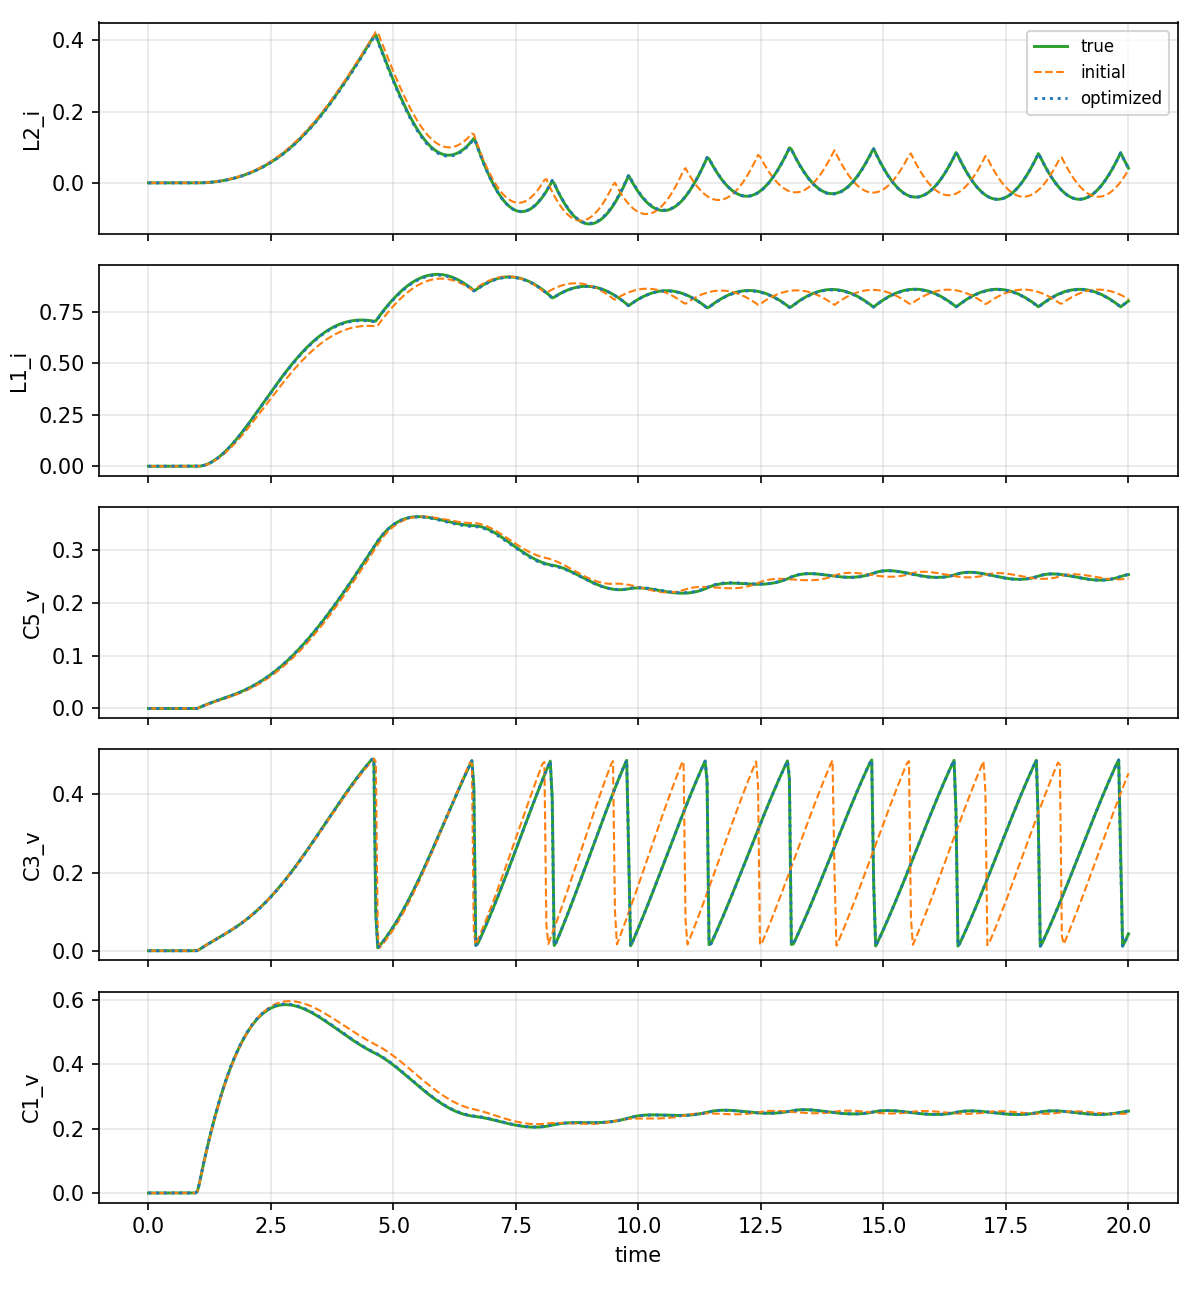
\includegraphics[width=\linewidth]{../results/optimization_cauer_events_adam_outputs.png}
    \caption{Implicit-AD route.}
  \end{subfigure}
  \hfill
  \begin{subfigure}[b]{0.48\linewidth}
    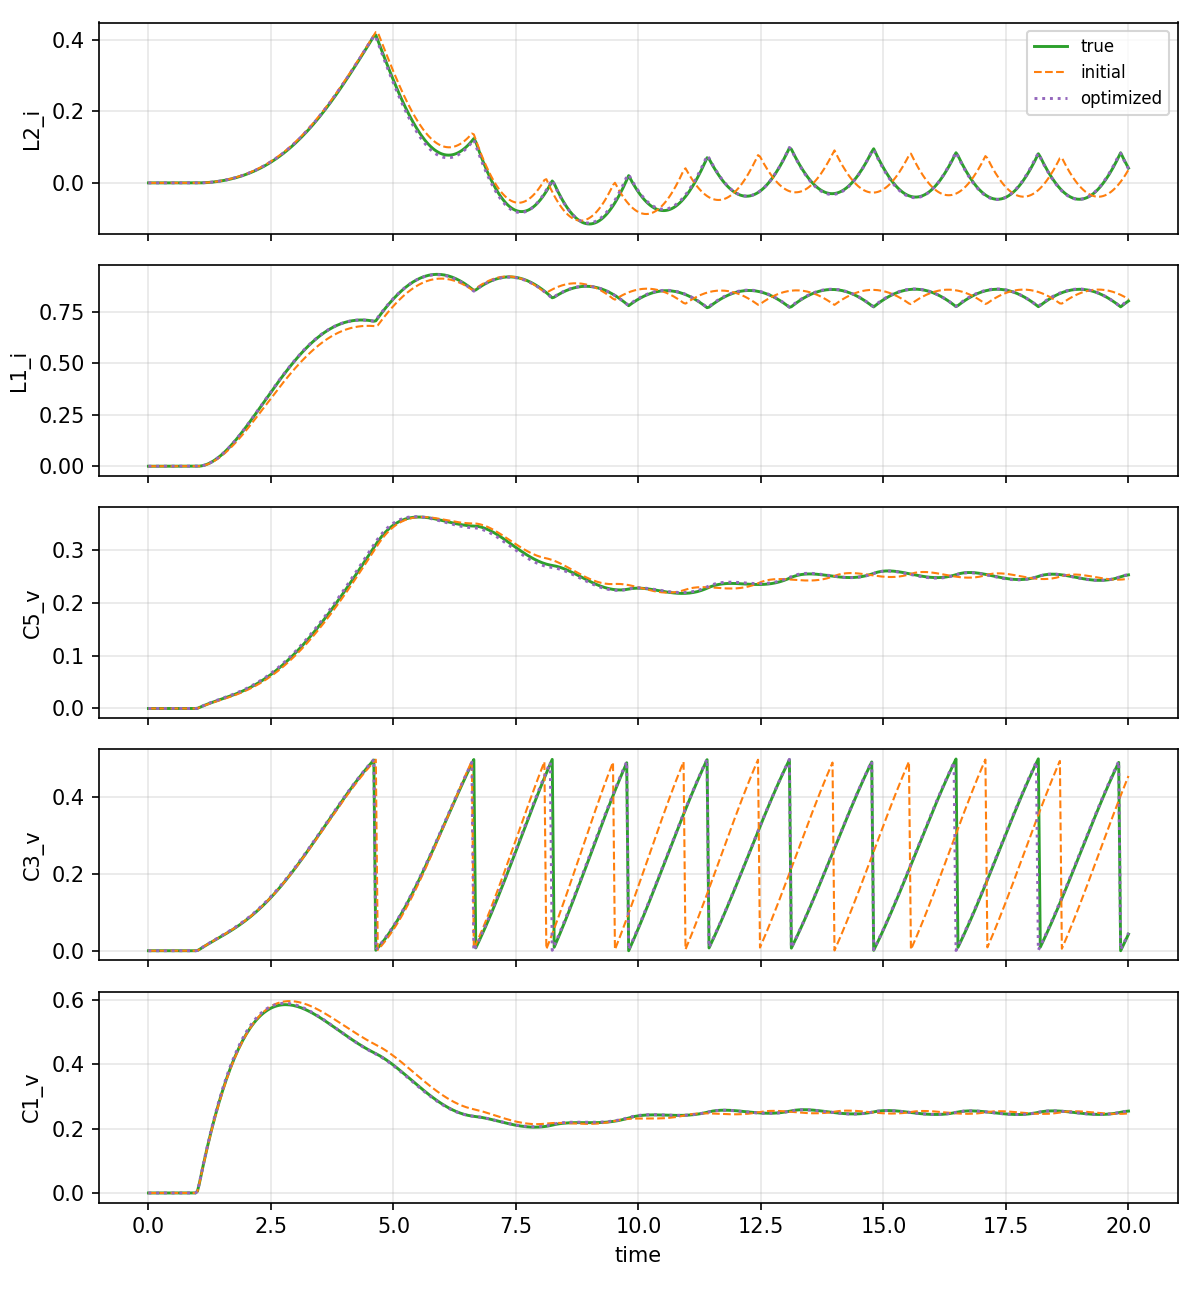
\includegraphics[width=\linewidth]{../results/optimization_cauer_events_da_outputs.png}
    \caption{Discrete-adjoint route.}
  \end{subfigure}
  \caption{Cauer ladder: optimized vs.\ true trajectories at the
  best-loss snapshot. Both routes capture the qualitative event
  structure; the AD route additionally matches the post-reset
  oscillation envelope.}
  \label{fig:cauer-overlays}
\end{figure}

\begin{figure}[t]
  \centering
  \begin{subfigure}[b]{0.48\linewidth}
    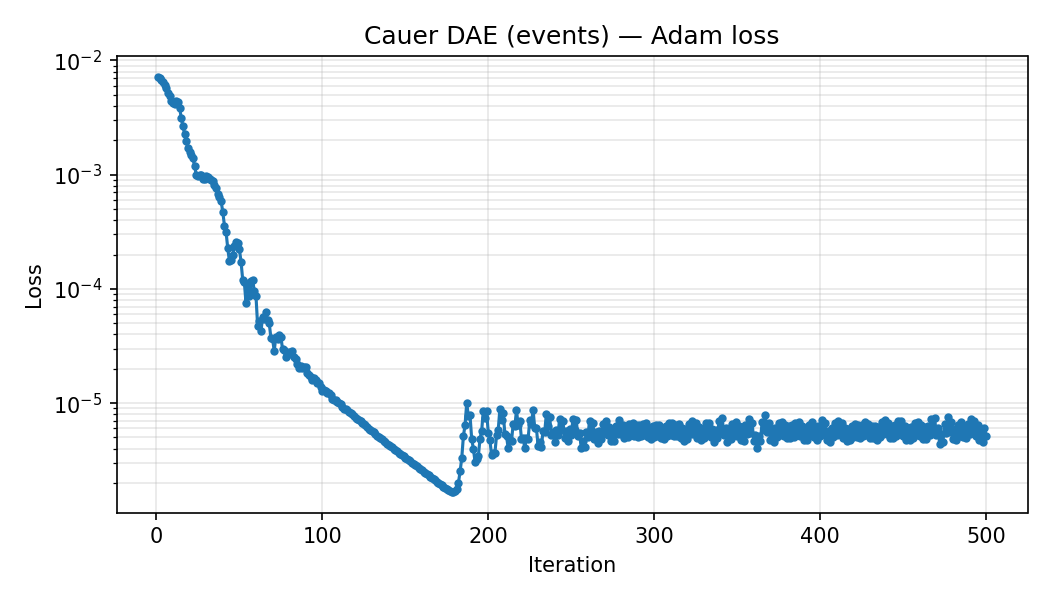
\includegraphics[width=\linewidth]{../results/optimization_cauer_events_adam_loss.png}
    \caption{AD loss history.}
  \end{subfigure}
  \hfill
  \begin{subfigure}[b]{0.48\linewidth}
    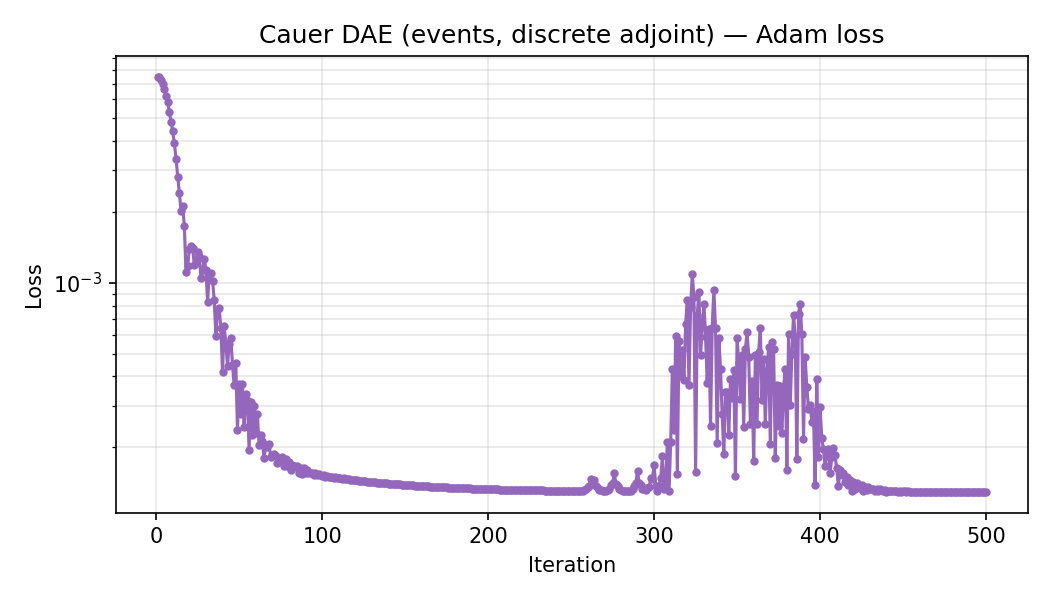
\includegraphics[width=\linewidth]{../results/optimization_cauer_events_da_loss.png}
    \caption{DA loss history.}
  \end{subfigure}
  \caption{Cauer ladder: Adam loss histories on log scale. The AD
  curve descends $\sim$5 decades whereas the DA curve plateaus at
  $\sim 10^{-4}$; the gap is consistent across the last
  $\sim 100$ iterations.}
  \label{fig:cauer-loss}
\end{figure}

\paragraph{Discussion.}
The accuracy gap between the two routes on this benchmark traces back
to two effects. First, the discrete-adjoint pipeline downsamples each
event-bounded segment to $\textsf{max\_pts}{=}50$ before forming the
trapezoidal-step Jacobians, so its gradient quality is bounded by the
adjoint mesh density rather than by the forward solver tolerance.
Second, the loss surface near the truth is anisotropic and dominated
by long-time-scale plateaus between events; with a uniform target
grid the trapezoidal Jacobians of the discrete adjoint accumulate a
small but coherent bias along the soft directions, observable here as
the residual error on $C_5$ and $C_1$. The implicit-AD pipeline does
not downsample, and its gradient inherits the diffrax tolerance
($\mathrm{rtol}{=}\mathrm{atol}{=}10^{-6}$) directly. The price is
that AD must hold the entire diffrax tape per segment in JAX memory;
on this 7-parameter system this is negligible, but it scales with the
number of state dimensions and the length of the dense-output tape, a
distinction that drives the next experiment.

% ------------------------------------------------------------------
\subsection{Multi-ball planar bouncing system: scaling with $N$}
\label{sec:exp:balls}

\paragraph{Setup.}
We consider a planar system of $N$ identical bouncing balls in a square
box of half-width $10$, with elastic collisions against the four walls
(restitution $e_b$) and inelastic ground impacts (restitution $e_g$).
The dynamics is an ODE with state-dependent events --- $4N+\binom{N}{2}$
event clauses for $N\in\{3,7,15\}$. We optimize three identifiable
parameters $\theta=(g, e_g, e_b)$ from a randomly biased start
($\pm 10\%$ log-uniform). All three identification routes share the
same $\mathrm{ncp}{=}500$ uniform target grid, the same Adam step
size, and the same convergence tolerance; the only differences are
how the gradient is obtained and which framework holds the autograd
tape:
\begin{description}
  \setlength{\itemsep}{2pt}
  \item[\texttt{jax\_ad}] our JAX/diffrax pipeline with implicit AD,
  same algebraic-solver custom-jvp as in \Cref{sec:exp:cauer}.
  \item[\texttt{jax\_da}] the JAX padded-discrete-adjoint pipeline of
  \Cref{sec:exp:cauer}, ported to ODE-with-events.
  \item[\texttt{pytorch\_ad}] PyTorch baseline using \texttt{torchdiffeq}
  with hand-written event-time root-finding, AD through the entire
  segmented integration tape.
\end{description}

\Cref{tab:balls-scaling} summarizes the result. Per-parameter
relative errors are reported as percentages, the final validation
loss is on a denser held-out target grid, and timing is total
wall-clock for the budget of iterations actually used (Adam runs to
the full budget unless the gradient-norm tolerance triggers).

\paragraph{Results.}

\begin{table}[t]
  \centering
  \small
  \caption{Multi-ball bouncing system with $N\in\{3,7,15\}$ balls.
  Per-parameter relative error in \%, final validation loss, and
  total wall-clock time. Budget: $300$ iters for $N\in\{3,7\}$ and
  $600$ iters for $N=15$. ``conv.'' marks gradient-tolerance
  convergence; otherwise the iteration budget was exhausted. Times
  measured on a single CPU thread.}
  \label{tab:balls-scaling}
  \begin{tabular}{llrrrrrrr}
    \toprule
    $N$ & Method & $|\Delta g|/g$ & $|\Delta e_g|/e_g$ & $|\Delta e_b|/e_b$ &
    Loss & Iter & Total time & ms/it \\
    \midrule
    \multirow{3}{*}{3}
      & \texttt{jax\_ad}     & \textbf{0.002} & \textbf{0.000} &
        \textbf{0.001} & \textbf{\num{1.40e-9}} & 300 & \SI{33.4}{\second}
        & 73.9 \\
      & \texttt{jax\_da}     & 0.27 & 1.16 & 0.16 & \num{9.38e-5} & 300
        & \SI{22.1}{\second} & 61.9 \\
      & \texttt{pytorch\_ad} & 0.003 & 0.001 & 0.003 & \num{3.89e-9} & 300
        & \SI{168.6}{\second} & 554.4 \\
    \midrule
    \multirow{3}{*}{7}
      & \texttt{jax\_ad}     & \textbf{0.002} & \textbf{0.001} &
        \textbf{0.001} & \textbf{\num{1.63e-9}} & 300 & \SI{33.4}{\second}
        & 71.2 \\
      & \texttt{jax\_da}     & 0.15 & 0.09 & 0.10 & \num{7.76e-6} & 300
        & \SI{84.0}{\second} & 254.8 \\
      & \texttt{pytorch\_ad} & 0.013 & 0.010 & 0.010 & \num{6.61e-8} & 300
        & \SI{525.5}{\second} & 1740.4 \\
    \midrule
    \multirow{3}{*}{15}
      & \texttt{jax\_ad}     & 0.07 & 0.19 & 0.42 & \num{1.35e-5} & 600
        & \SI{77.2}{\second} & 110.1 \\
      & \texttt{jax\_da}     & 0.21 & 2.67 & 4.04 & \num{9.28e-4} & 495
        \textsuperscript{conv.} & \SI{595.7}{\second} & 1157.5 \\
      & \texttt{pytorch\_ad} & \textbf{0.000} & \textbf{0.005} &
        \textbf{0.001} & \textbf{\num{3.88e-8}} & 423 \textsuperscript{conv.}
        & \SI{2826.9}{\second} & 6652.2 \\
    \bottomrule
  \end{tabular}
\end{table}

\begin{figure}[t]
  \centering
  \begin{subfigure}[b]{0.32\linewidth}
    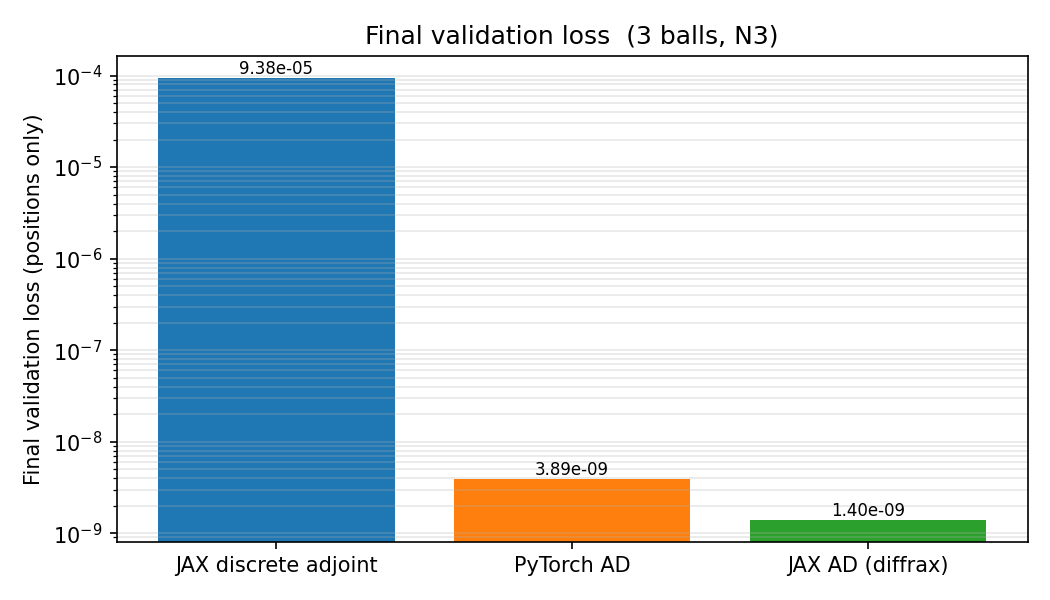
\includegraphics[width=\linewidth]{../results/benchmark_three_N3_validation_loss.png}
    \caption{$N=3$.}
  \end{subfigure}
  \hfill
  \begin{subfigure}[b]{0.32\linewidth}
    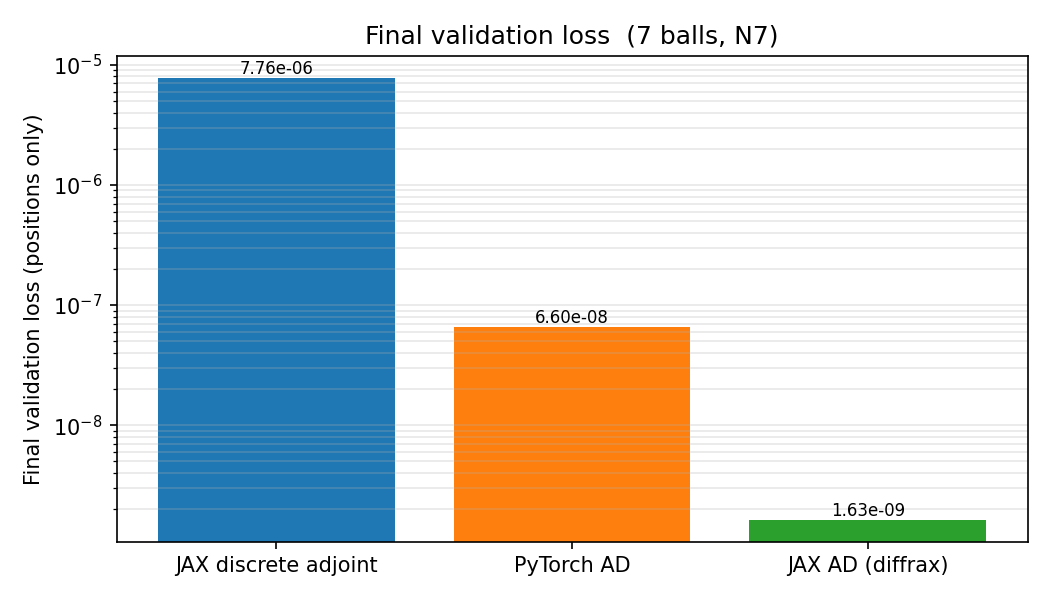
\includegraphics[width=\linewidth]{../results/benchmark_three_N7_validation_loss.png}
    \caption{$N=7$.}
  \end{subfigure}
  \hfill
  \begin{subfigure}[b]{0.32\linewidth}
    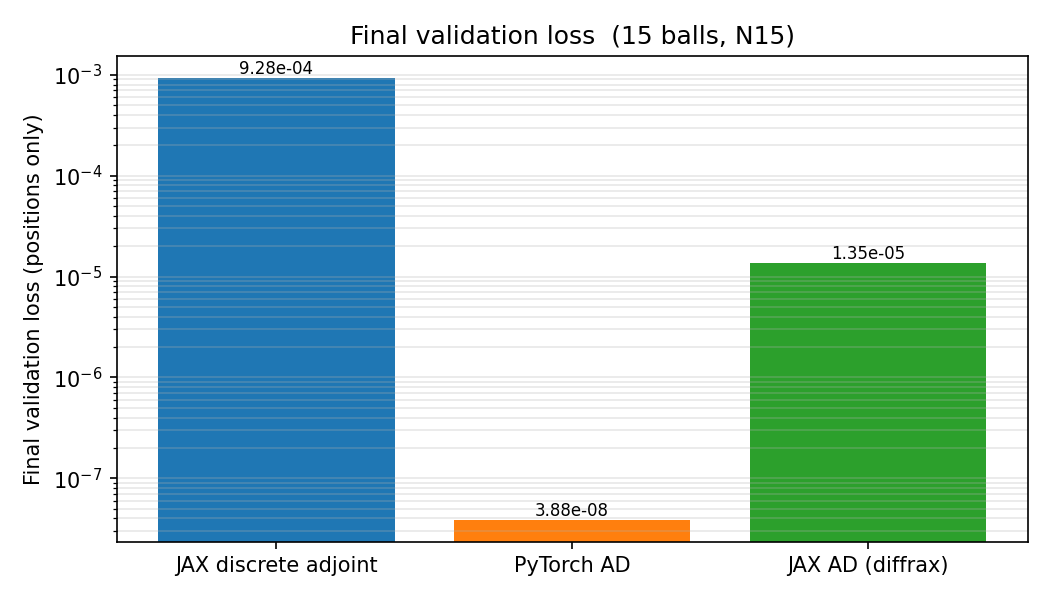
\includegraphics[width=\linewidth]{../results/benchmark_three_N15_validation_loss.png}
    \caption{$N=15$.}
  \end{subfigure}
  \caption{Bouncing balls: validation loss vs.\ iteration for each
  route at $N\!\in\!\{3,7,15\}$. The PyTorch-AD baseline reaches the
  lowest steady-state loss in every case; our JAX-AD pipeline is
  within an order of magnitude (and beats PyTorch at $N\!\in\!\{3,7\}$)
  while running an order of magnitude faster
  (cf.\ \Cref{tab:balls-scaling}).}
  \label{fig:balls-loss}
\end{figure}

\begin{figure}[t]
  \centering
  \begin{subfigure}[b]{0.32\linewidth}
    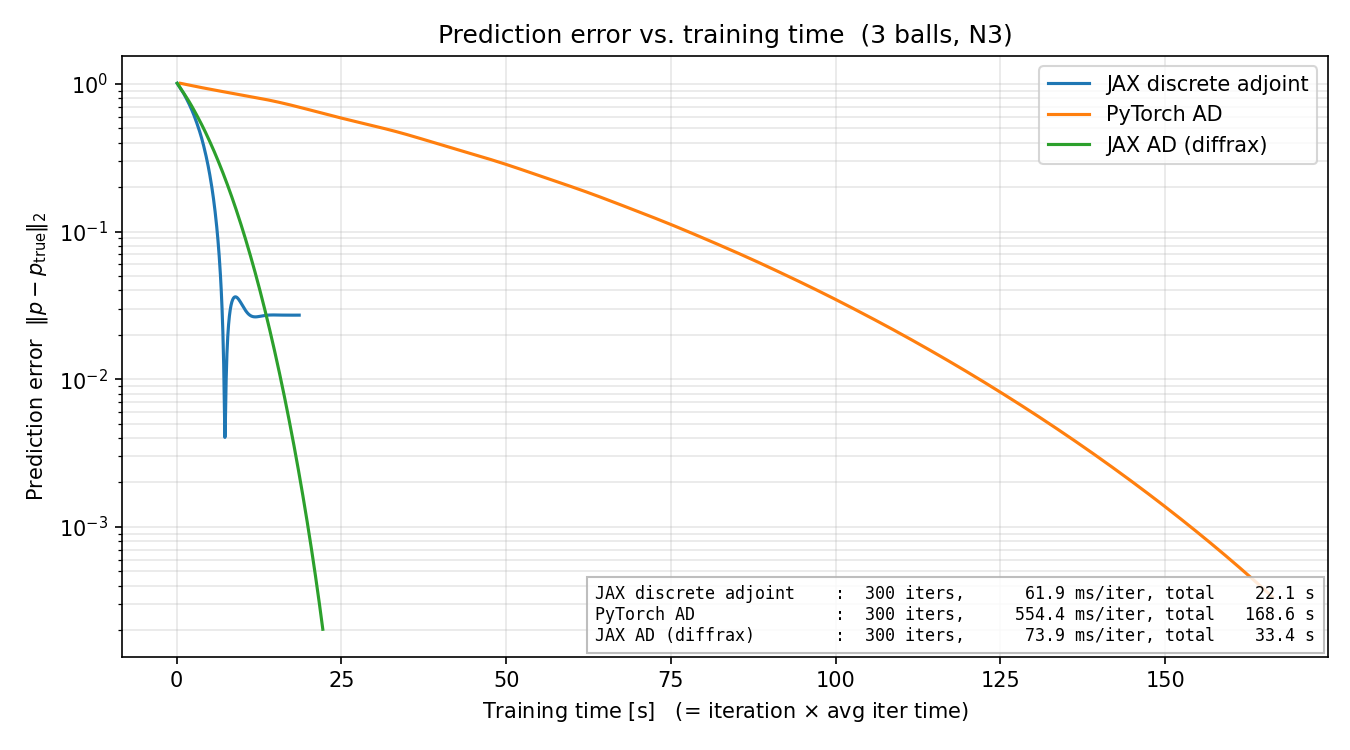
\includegraphics[width=\linewidth]{../results/benchmark_three_N3_prediction_error_vs_time.png}
    \caption{$N=3$.}
  \end{subfigure}
  \hfill
  \begin{subfigure}[b]{0.32\linewidth}
    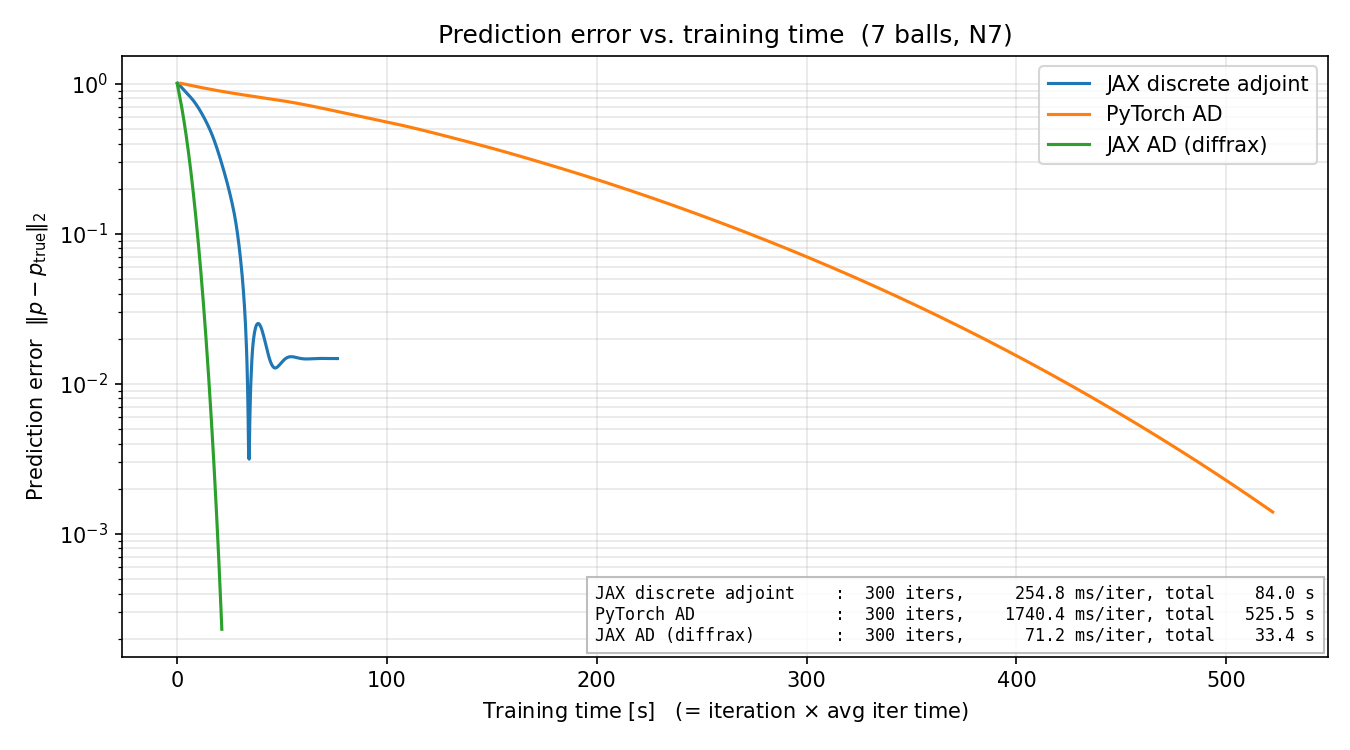
\includegraphics[width=\linewidth]{../results/benchmark_three_N7_prediction_error_vs_time.png}
    \caption{$N=7$.}
  \end{subfigure}
  \hfill
  \begin{subfigure}[b]{0.32\linewidth}
    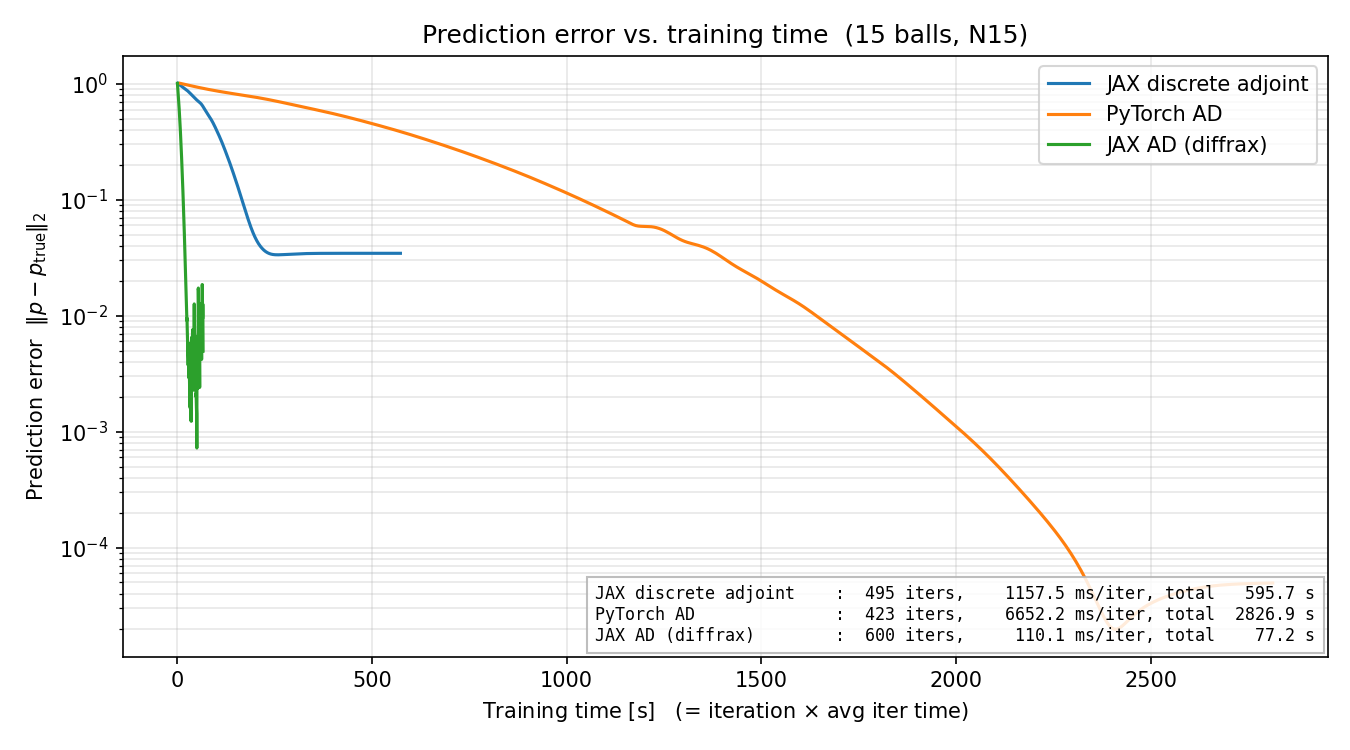
\includegraphics[width=\linewidth]{../results/benchmark_three_N15_prediction_error_vs_time.png}
    \caption{$N=15$.}
  \end{subfigure}
  \caption{Bouncing balls: prediction error vs.\ wall-clock time. The
  horizontal axis exposes the throughput differential: the JAX-AD curve
  reaches the same accuracy plateau as the PyTorch-AD curve in
  $5\!\times$ to $35\!\times$ less wall-clock time across the three
  problem sizes.}
  \label{fig:balls-time}
\end{figure}

\paragraph{Discussion.}
Three observations stand out.

\emph{(i) Per-iteration scaling with $N$.} The JAX-AD pipeline is the
flattest: $74 \!\to\! 71 \!\to\! 110$~ms/iter as $N$ goes from $3$ to
$15$. JIT compilation amortizes across iterations, so the marginal
cost is dominated by the diffrax forward and the segment-wise solve;
both stay vectorized in $N$. The PyTorch-AD baseline scales steeply
($554 \!\to\! 1740 \!\to\! 6652$~ms/iter, roughly $3\times$ per
$N\!\to\!2N$), reflecting the unfused per-event-segment work and the
overhead of \texttt{torchdiffeq}'s adaptive stepper rebuilding its
graph each call. The JAX-DA pipeline sits between the two and
inherits the discrete-adjoint cost of building per-step Jacobians,
which scales with the segment count and hence with the event density.

\emph{(ii) Accuracy/throughput frontier.} At $N\!\in\!\{3,7\}$, our
JAX-AD pipeline strictly dominates: it reaches a lower loss (by
$\sim\!2\!\times$) in $\sim\!5\!\times\text{--}16\!\times$ less wall
time. At $N=15$ the comparison flips: PyTorch-AD reaches
$3.9\!\times\!10^{-8}$ versus JAX-AD's $1.4\!\times\!10^{-5}$ but at
$37\!\times$ the cost. Whether the extra accuracy is worth it depends
on the downstream task; for parameter identification under noisy
measurements, the JAX-AD result is well within the noise floor of any
realistic measurement model.

\emph{(iii) When the discrete adjoint trails.} The JAX-DA results
mirror the Cauer experiment: the route is competitive on small
problems but the gradient bias induced by the per-segment
trapezoidal mesh and the uniform target grid grows with $N$, ending
at $\sim\!4\%$ on $e_b$ at $N=15$. We discuss in
\Cref{sec:limitations} that this is not a fundamental property of
the discrete adjoint --- finer per-segment meshes would close the
gap --- but it is a property of the padded fixed-shape JIT regime
that makes the route fast on small problems.

% --- end of file
